\documentclass[a4paper, 12pt]{article}%тип документа

%отступы
\usepackage[left=2cm,right=1cm,top=2cm,bottom=3cm,bindingoffset=0cm]{geometry}
\setlength{\parindent}{5ex}

%Русский язык
\usepackage[T2A]{fontenc} %кодировка
\usepackage[utf8]{inputenc} %кодировка исходного кода
\usepackage[english,russian]{babel} %локализация и переносы

%Вставка картинок
\usepackage{graphicx}
\graphicspath{{pictures/}}
\DeclareGraphicsExtensions{.pdf,.png,.jpg,}
\usepackage{wrapfig}

%Графики
\usepackage{pgfplots}
\pgfplotsset{compat=1.9}

%Математика
\usepackage{amsmath, amsfonts, amssymb, amsthm, mathtools}

%Таблицы
\usepackage{longtable} 
\usepackage{float}

%Римские цифры
\newcommand{\RomanNumeralCaps}[1]{\uppercase\expandafter{\romannumeral#1}}

\usepackage{multirow}


\begin{document}
	\begin{titlepage}
		\begin{center}
			\textsc{Федеральное государственное автономное образовательное учреждение высшего образования«Московский физико-технический институт (национальный исследовательский университет)»\\[5mm]
			}
			
			\vfill
			
			\textbf{Отчёт по лабораторной работы 4.7.3\\[3mm]
				ИЗУЧЕНИЕ
				ПОЛЯРИЗОВАННОГО СВЕТА 
				\\[50mm]
			}
			
		\end{center}
		
		\hfill
		\begin{minipage}{.5\textwidth}
			Выполнил студент:\\[2mm]
			Сериков Василий Романович\\[2mm]
			группа: Б03-102\\[5mm]
			
		\end{minipage}
		\vfill
		\begin{center}
			Москва, 2023 г.
		\end{center}
		
	\end{titlepage}
	
	\newpage
	\setcounter{page}{2}
	
	\textbf{Аннотация}\\
	
	
	\textbf{Цель работы: }\\
	Ознакомление с методами получения и анализа поляризованного света.\\
	
	\textbf{В работе используется: }\\
	Оптическая скамья с осветителем; зеленый светофильтр; два поляроида; черное зеркало; полированная эбонитовая пластинка; стопа стеклянных пластинок; слюдяные пластинки разной толщины; пластинки в 1/4 и 1/2 длины волны; пластинка
	в одну длину волны для зеленого света (пластинка чувствительного
	оттенка).\\
	
	\textbf{Теория: }\\
	
	\textit{Определение направления разрешённой плоскости колебаний поляроида}\\
	
	Определить направление разрешённых колебаний поляроида проще всего с помощью чёрного зеркала.
	
	При падении света на отражающую поверхность под углом Брюстера, свет в отражённом луче почти полностью поляризован, а вектор E
	параллелен отражающей поверхности ("<правило иголки">). Луч света,
	прошедший поляроид и отразившийся от чёрного зеркала, имеет минимальную интенсивность при выполнении двух условий: во-первых, свет
	падает на отражающую поверхность под углом Брюстера и, во-вторых,
	в падающем пучке вектор E лежит в плоскости падения.
	
	Вращая поляроид вокруг направления луча и чёрное зеркало вокруг
	оси, перпендикулярной лучу, методом последовательных приближений
	можно добиться минимальной яркости луча, отражённого от зеркала,
	и таким образом определить разрешённое направление поляроида.
	
	Измеряя угол поворота зеркала (угол Брюстера), нетрудно определить коэффициент преломления материала, из которого изготовлено
	зеркало. Описанный метод часто используется для измерения коэффициента преломления непрозрачных диэлектриков.\\
	\begin{wrapfigure}{r}{0.3\linewidth} 
		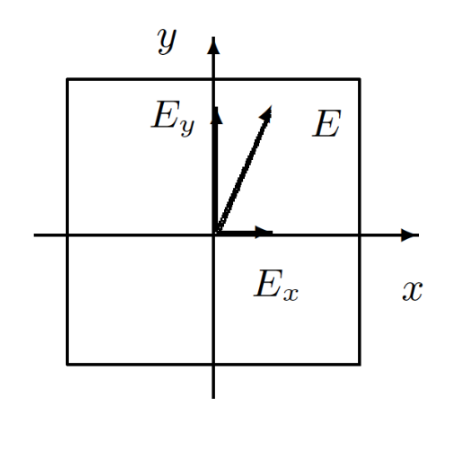
\includegraphics[width=\linewidth]{1}
		\caption{Разложение линейно поляризованного света по главным направлениям двоякопреломляющей пластинки}
		\label{ris 1}
	\end{wrapfigure}
	
	\textit{Получение эллиптически поляризованного света}\\
	
	Эллиптически поляризованный свет можно получить из линейно поляризованного с
	помощью двоякопреломляющих кристаллических пластинок.
	
	Двоякопреломляющая пластинка имеет два взаимно перпендикулярных главных направления, совпадающих с осями эллипсоида диэлектрической проницаемости. Волны, поляризованные вдоль главных направлений, распространяются в пластинке с разными скоростями, не изменяя характера своей поляризации. Эти волны называются главными. Мы будем обозначать показатели преломления для главных волн через $ n_x $ и $ n_y $, где $ x $ и $ y $ --- главные направления кристаллической пластинки (рис. 1).
	
	\newpage
	
	Пусть на пластинку падает линейно поляризованная волна, электрический вектор которой ориентирован под некоторым углом $ \alpha $ к оси
	$ x $. Разложим вектор $ \mathbf{E} $ на составляющие $ E_x $ и $ E_y $. На входе пластинки $ E_x $ и $ E_y $ находятся в фазе. На выходе из-за разности скоростей между ними появляется разность хода $ d(n_x - n_y) $, при этом сдвиг фаз определяется соотношением
	
	\begin{equation}\label{}
		\Delta \phi =  \dfrac{2\pi}{m} = k d(n_x - n_y)
	\end{equation}
	Как уже отмечалось, при сложении двух взаимно перпендикулярных колебаний, обладающих некоторым сдвигом фаз, образуется колебание, поляризованное по эллипсу.
	
	\begin{wrapfigure}{l}{0.35\linewidth}
		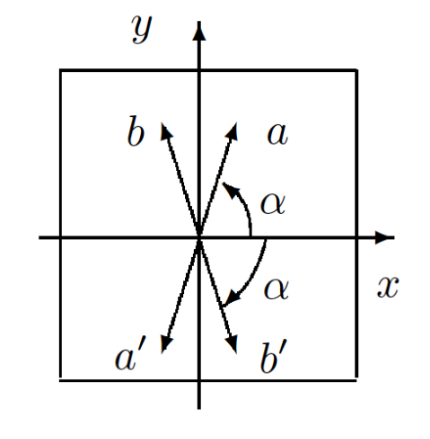
\includegraphics[width=\linewidth]{2}
		\caption{Поворот направления колебаний с помощью пластинки в $ \lambda / 2 $}
		\label{ris 2}
	\end{wrapfigure}
	
	
	Рассмотрим практически важные частные случаи.
	
	\begin{enumerate}
		
		\item Пластинка даёт сдвиг фаз $ 2\pi $ (пластинка в длину волны $ \lambda $). В результате сложения волн на выходе пластинки образует-
		ся линейно поляризованная волна с тем же направлением колебаний, что и в падающей волне.
		
		\item Пластинка даёт сдвиг фаз $ \pi $ (пластинка в полдлины волны $ \lambda / 2 $). На выходе пластинки снова образуется линейно поляризованная волна. Направление $ bb' $ колебаний этой волны повёрнуто относительно направления $ aa' $ колебаний падающей волны (рис. 2). Как нетрудно сообразить, направление $ bb' $ является зеркальным отображением направления $ aa' $ относительно одного из главных направлений пластинки. Такую пластинку используют для поворота направления колебаний линейно поляризованного света.
		
		\item Пластинка создаёт между колебаниями сдвиг фаз $ \pi/2 $ (пластинка
		в четверть длины волны). При сложении двух взаимно перпендикулярных колебаний, имеющих разность фаз $ \pi/2 $, образуется эллипс, главные оси которого совпадают с координатными осями $ x $ и $ y $. При равенстве амплитуд возникает круговая поляризация.
		
	\end{enumerate}
	
	Следует отметить, что, говоря о пластинках $ \lambda , \lambda/2, \lambda/4  $ и т. д., всегда подразумевают какую-либо вполне определённую монохроматическую
	компоненту (например, пластинка $ \lambda/2 $ для зелёного света). Если на двоякопреломляющую пластинку падает не монохроматический свет, то на
	выходе из неё для разных спектральных компонент эллипсы поляризации будут различными.\\
	
	\textit{Анализ эллиптически поляризованного света}\\
	
	Анализ эллиптически поляризованного света сводится к нахождению главных осей
	эллипса поляризации и к определению направления вращения электрического вектора.
	
	Главные оси эллипса поляризации определяются с помощью анализатора по максимуму и минимуму интенсивности проходящего света.
	Направление вращения электрического вектора может быть найдено
	с помощью пластинки в четверть длины волны, для которой известно,
	какая из главных волн, $ E_x $ или $ E_y $, имеет б\'{o}льшую скорость распространения (и соответственно меньшее значение показателя преломления).
	
	Выберем для определённости координатные оси x и y на пластинке
	так, чтобы $ nx < ny $. В этом случае главная волна $ E_x $ имеет большую
	скорость распространения. Поместим такую пластинку на пути эллиптически поляризованного света и совместим главные направления пластинки $ \lambda/4 $ с главными осями эллипса поляризации. На выходе из этой
	пластинки сдвиг фаз между $ E_x $ и $ E_y $ вместо $ \pi/2 $ станет равным ну-
	лю или $ \pi $. Свет окажется линейно поляризованным. Из двух возможных значений сдвига фаз, 0 или $ \pi $, реализуется одно: то, которое соответствует имеющемуся в волне направлению вращения электрического вектора.
	
	Рассмотрим, например, случай, когда электрический вектор в эллиптически поляризованной волне вращается против часовой стрелки,
	если смотреть навстречу лучу. В этом случае, очевидно, в волне, падающей на пластинку в $ \lambda/4 $, колебание $ E_y $ отстаёт по фазе на $ \pi/2 $ от
	колебания $ E_x $. При прохождении через пластинку разность фаз увеличивается до $ \pi $. Таким образом на выходе из пластинки возникают линейно поляризованные волны со сдвигом фаз $ \pi $. Сложение этих волн
	даёт плоскополяризованную волну, электрический вектор которой рас-
	полагается во втором и четвёртом квадрантах координатной системы
	$ x, y $.
	
	Рассуждая аналогичным образом, найдём, что при вращении электрического вектора по часовой стрелке направление колебаний в линейно поляризованной волне, выходящей из пластинки, располагается в первом и третьем квадрантах. Определяя направление колебаний на выходе из пластинки с помощью поляроида, можно, таким образом, определить характер эллиптической поляризации (вращение против или по часовой стрелке).\\
	
	\textit{Пластинка чувствительного оттенка}\\
	
	\begin{wrapfigure}{l}{0.35\linewidth}
		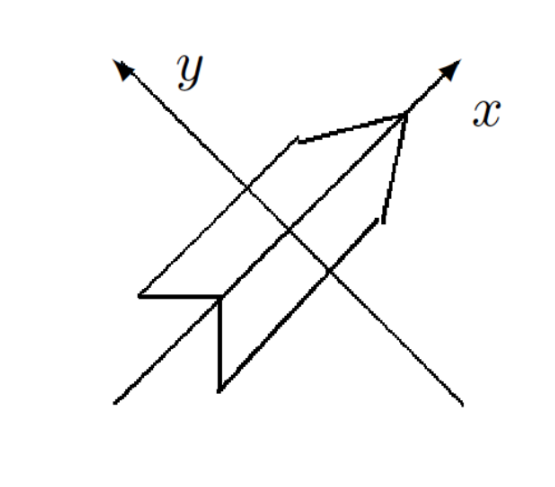
\includegraphics[width=\linewidth]{3}
		\caption{Пластинка
			чувствительного
			оттенка}
		\label{ris 3}
	\end{wrapfigure}
	
	Выше предполагалось известным, какому из двух главных направлений пластинки в четверть длины волны соответствует большая скорость распространения света.
	Установить это можно различными способами, например с помощью
	пластинки чувствительного оттенка (так называют пластинку в $ \lambda $
	для зелёной спектральной компоненты, $ \lambda = 560 $ нм).
	
	Пластинка имеет форму стрелы (рис. 3), вдоль оси которой расположено главное направление, соответствующее большей скорости распространения.
	
	Если пластинка чувствительного оттенка помещена между скрещенными поляроидами и главные направления пластинки не параллельны
	направлениям разрешённых колебаний поляроидов, то при освещении
	белым светом пластинка кажется окрашенной в лилово-красный цвет.
	Это объясняется тем, что зелёная компонента линейно поляризованного света при прохождении пластинки не меняет поляризации и задерживается вторым поляроидом. Для красной и фиолетовой компонент
	пластинка создаёт сдвиг фаз, несколько отличный от $ 2\pi $. На выходе
	из пластинки красная и фиолетовая компоненты оказываются поэтому
	эллиптически поляризованными и частично проходят через второй поляроид. Таким образом, в известном смысле наблюдаемый в указанном
	опыте цвет пластинки дополнителен к зелёному.
	
	Если между скрещенными поляроидами поместить пластинку чувствительного оттенка
	($ \lambda $) и пластинку в $ \lambda/4 $ так, чтобы их главные
	направления совпадали, цвет пластинки изменится. Если у пластинки чувствительного оттенка и пластинки в $ \lambda/4  $совпадут главные направления, соответствующие большей скорости распространения, то разность хода между $ E_x $ и $ E_y $ для зелёного света составит уже $ 5\lambda/4 $. Это соответствует разности хода в $ \lambda $ для света с большей длиной волны, т. е. для "<более красного"> света. При освещении
	этих пластинок (напомним, что они расположены между скрещенными поляроидами) белым светом теперь погасится не зелёная, а красная
	часть спектра, и проходящий свет будет казаться зеленовато-голубым.
	Если же главные направления, соответствующие большей скорости распространения, у пластинки чувствительного оттенка и у пластинки
	в $ \lambda/4 $ окажутся перпендикулярными, то проходящий свет приобретёт
	оранжево-желтую окраску (погасится фиолетово-голубая часть спектра).
	
	Изменение цвета позволяет, таким образом, определить, какое из
	главных направлений пластинки в $ \lambda/4 $ соответствует большей скорости
	распространения.\\
	
	\textit{Интерференция поляризованных лучей}\\
	
	\begin{wrapfigure}{r}{0.35\linewidth}
		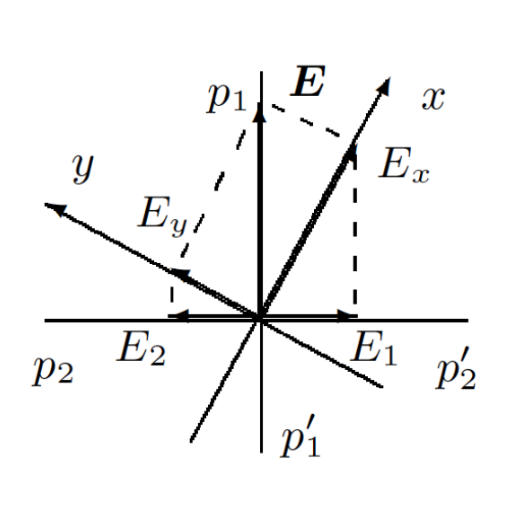
\includegraphics[width=\linewidth]{4}
		\caption{К объяснению интерференции
			поляризованных лучей}
		\label{ris 4}
	\end{wrapfigure}
	
	
	Тонкие двоякопреломляющие пластинки, помещённые между поляроидами, кажутся окрашенными. Эта окраска может быть истолкована как результат интерференции поляризованных лучей. На рис. 4 представлена схема для
	случая скрещенных поляроидов.
	
	Здесь $ p1p'1 $ --- разрешённое направление колебаний поляризатора
	(первого поляроида); $ x, y $ --- координатная система, связанная с главны-
	ми направлениями двоякопреломляющей пластинки; $ p2p'2 $ --- разрешённое направление колебаний анализатора (второго поляроида). Волны
	$ E_x  $ и $ E_y $ на выходе из пластинки когерентны, но не могут интерферировать, так как $ E_x \perp  E_y $. Волны $ E_1 $ и $ E_2 $ на выходе второго поляроида
	также являются когерентными и к тому же поляризованы в одной плоскости. Эти волны интерферируют между собой. Результат интерференции определяется зависящим от длины волны сдвигом фаз между $ E_1 $
	и $ E_2 $. В результате интерференции поляризованных лучей пластинка, освещаемая белым светом, кажется окрашенной.
	
	Если поворачивать двоякопреломляющую пластинку, расположенную между
	скрещенными поляроидами, то соотношение амплитуд волн $ E_1 $ и $ E_2 $ и разность фаз между ними не изменяются. Это означает, что цвет пластинки при её поворотах не меняется, а меняется только интенсивность света. За один оборот пластинки интенсивность четыре раза обращается в нуль --- это происходит при совпадении главных направлений
	$ x $ и $ y $ с разрешёнными направлениями колебаний поляроидов.
	
	Если же двоякопреломляющую пластинку оставить неподвижной, а
	второй поляроид повернуть так, чтобы разрешённые направления $ p1p'1 $
	и $ p2p'2 $ совпали, то волны $ E_1 $ и $ E_2 $ приобретают дополнительный фазовый сдвиг на $ \pi $ для всех спектральных компонент; при этом их амплитуды изменятся так, что цвет пластинки изменится на дополнительный. \\
	\newpage
	
	\textbf{Ход работы: }\\
	
	\textit{Определение разрешённых направлений поляроидов}\\
	\begin{wrapfigure}{r}{0.35\linewidth}
		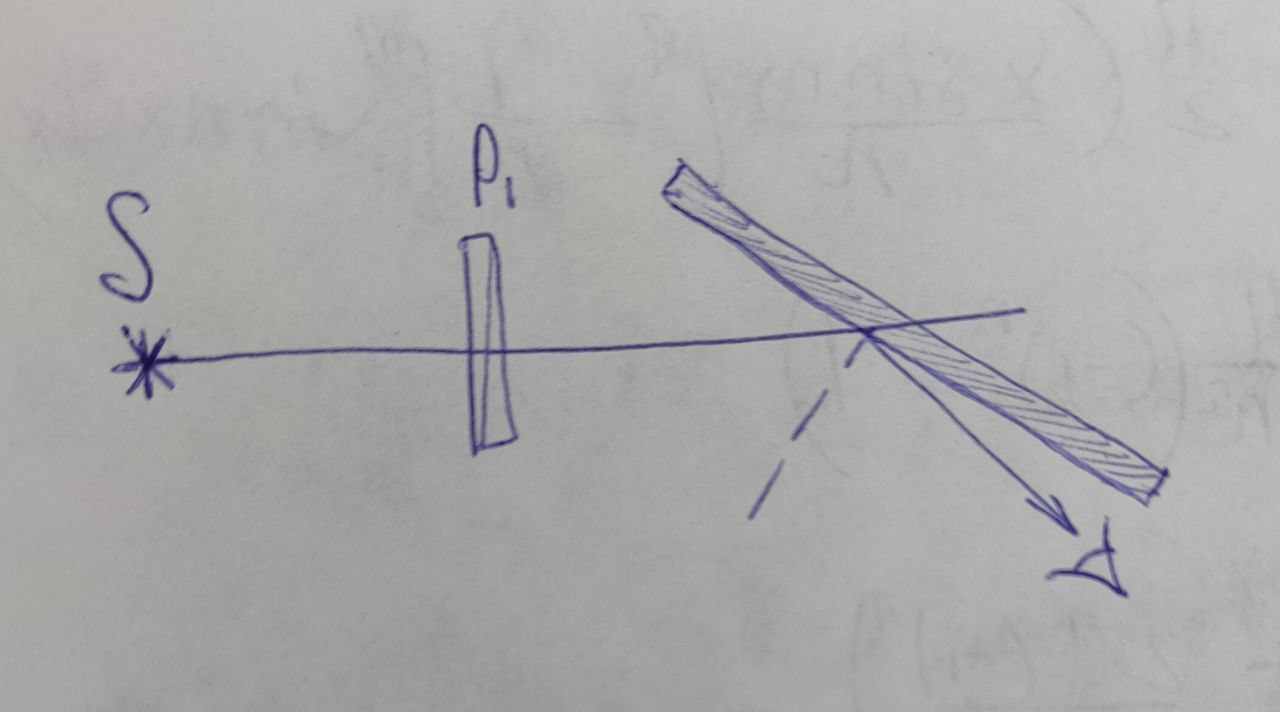
\includegraphics[width=\linewidth]{first}
		\caption{ход лучей в зеркале через поляроид}
	\end{wrapfigure}
	
	С помощью черного зеркала и осветителя можно определить разрешенное направление. Поворачивая поляроид вокруг направления луча, добьемся наименьшей яркости отражённого пятна. Оставим поляроид в этом положении и вращением зеркала вокруг вертикальной оси снова добьемся минимальной интенсивности отражённого луча. Таким образом получим значение угла поворота поляроида при котором пропускается одно направление.\\
	
	\textit{Определение угла Брюстера для эбонита}\\
	
	Так как направление разрешённых колебаний поляроида P1 горизонтально, то найдем угол поворота эбонита $\phi $, при котором интенсивность отражённого луча минимальна -- это угол Брюстера. Аналогично рассчитаем угол Брюстера, добавив в систему светофильтр. По полученным результатам рассчитаем показатель преломления эбонита.
	
	$$ \tg \phi = n => n = \tg(56\circ) = 1,5 \pm 0,1 - \text{без фильтра}$$
	
	$$ \tg \phi = n => n = \tg(59\circ) = 1,7 \pm 0,1 - \text{с фильтром}$$\\
	
	
	\textit{Исследование стопы}\\
	\begin{wrapfigure}{r}{0.35\linewidth}
		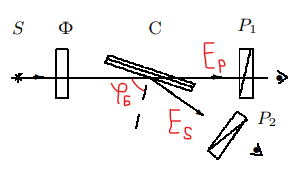
\includegraphics[width=\linewidth]{stopa}
		\caption{ход лучей в стопе}
	\end{wrapfigure}
	
	Поставим стопу стеклянных пластинок вместо эбонитового зеркала
	и подберем для неё такое положение, при котором свет падает на стопу под углом Брюстера. Осветим стопу неполяризованным светом и, рассматривая через поляроиды свет, отражённый от стопы, определим ориентацию вектора E в отражённом луче.\\
	
	
	\begin{wrapfigure}{l}{0.35\linewidth}
		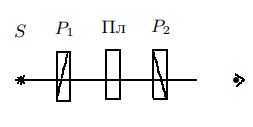
\includegraphics[width=\linewidth]{()}
		\caption{Пластина и два поляроида}
	\end{wrapfigure}
	
	\textit{Определение главных плоскостей двоякопреломляющих пластин}\\
	
	Вращая пластинку вокруг направления луча и наблюдая за интенсивность света, проходящего сквозь второй поляроид, определим, при каком условии главные направления пластинки совпадают с разрешёнными направлениями поляроидов.
	
	1) Свет распространяется вдоль оптической оси (при этом поляризация будет перпендикулярна оптической оси), тогда показатель преломления будет одинаковый для всех поляризаций, и кристалл в этом случае не отличается от изотропной среды, а между обыкновенной и необыкновенной волнами нет разницы.
	
	2) Свет распространяется перпендикулярно оптической оси. Тогда поляризацию можно разложить на две проекции — параллельную оптической оси и перпендикулярную. Эффективный показатель преломления будет разным для света двух ортогональных поляризаций, и при прохождении через слой (пластинку) материала может наблюдаться сдвиг по фазе между двумя компонентами. Если исходная поляризация линейная и ориентирована либо полностью вдоль, либо полностью перпендикулярно оптической оси, то на выходе из пластинки она не изменится. Однако, если исходно свет поляризован под углом к оптической оси, либо поляризация эллиптическая или циркулярная, то при прохождении через пластинку из одноосного кристалла поляризация может измениться из-за сдвига по фазе между компонентами. Сдвиг зависит от толщины пластинки, разницы между показателями преломления и длины волны света.
	
	Пусть угол между поляризацией и оптической осью равен 45$\circ$. Если толщина пластинки такова, что на выходе из неё одна поляризация на четверть волны отстаёт от другой, то исходная линейная поляризация превратится в круговую (такая пластинка называется $\lambda/4$), если фаза одного луча отстанет от фазы другого луча на половину длины волны, то свет останется линейно поляризованным, но плоскость поляризации повернётся на некоторый угол, значение которого зависит от угла между плоскостью поляризации падающего луча и плоскостью главной оптической оси (такая пластинка называется $\lambda/2$).\\
	
	
	\textit{Определение направления вращения светового вектора в
		эллиптически поляризованной волне}\\

	Электрический вектор в эллиптически поляризованной волне вращается против часовой стрелки, если
	смотреть навстречу лучу. В этом случае, в волне, падающей
	на пластинку в $\lambda/4$, колебание
	$E_y$ отстает по фазе на $\pi/2$ от
	колебания $E_x$. При прохождении через пластинку разность фаз увеличивается до $\pi$. На выходе из пластинки, таким образом, возникают линейно поляризованные волны со сдвигом фаз $\pi$. Сложение этих волн дает плоскополяризованную волну, электрический вектор
	которой располагается во втором и четвертом квадрантах координатной системы x, y.
	\begin{figure}[H]
		\begin{center}
			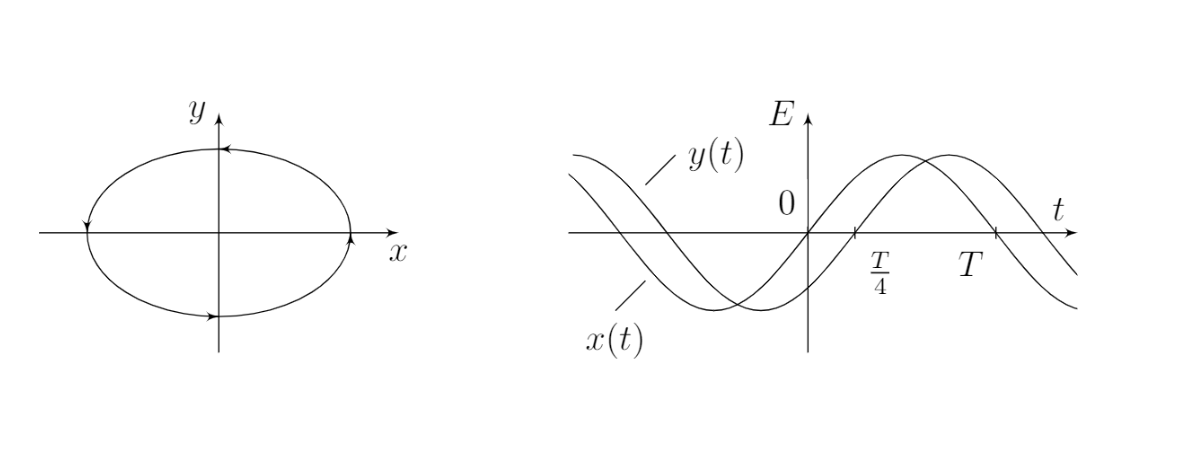
\includegraphics[width = 0.68\textwidth]{ellips}
			\caption{Эллипс поляризации и график синусоид}
		\end{center}
	\end{figure}
	
	\textbf{Выводы: }\\
	В данной работе мы познакомились с методами получения и анализа поляризованного света. Находили объяснения различным явлениям поляризации света в поляроидах и различных пластинках.
	
	
	
	
	
	
	
	
	
	
	
	
	
	
	
	
	
	
	
	
	\end{document}